\section{GaN sensors with ROIC}\label{sec:GaN_sensors_with_ROIC}
After the ROIC is characterized with constant controlled current sources, the next step is to attach it to the GaN sensors. The target range of operating voltages for the GaN sensors is 0 to -$100\,V$. The primary interest lies in the I/V characteristics of the system. Because the same cations need to be performed all the time, it is worth to automate the setup one step further to save time.

\subsection{Setup}\label{ssec:GaN_setup}
In order to automate the measuring process further, the oscilloscope is connected to the laptop by cable, and directly controlled by \texttt{labVIEW}. \texttt{LabVIEW} automatically acquires the required waveforms from the oscilloscope, and calculates the slope in real time. This action is repeated and used to accumulate data points for the $I/V$ curve. When the  program is finished, the processed data is stored. A bashscript collects all the data and calls \texttt{octave-cli} to put the results in a plot. There are two ways, that have been used to controll the bias voltage of the GaN sensors. The first method is to use the arbitrary function generator (AFG) on the oscilloscope to generate a DC voltage between $-2.5$ and $2.5\,V$. A voltage amplifier with a gain of 10 is then used to achieve a range of $-25$ to $25\,V$ that is directly controllable in \texttt{labVIEW}. This allows \texttt{labVIEW} to automatically sweep the bias voltage. However, the range of $-25$ to $25\,V$ does not cover the target bias voltage range. Therefore, in order to increase the range further, a second method is used. This time the bias voltage is controlled manually with a voltage source. The oscilloscope measures both the input and output voltage. \texttt{LabVIEW} then calculates $x$ and $y$ co\"ordinates repeatedly. This method provides the operator with full control over which part of the $I/V$ curve is measured.

\subsection{Calculation of current}
The calculation of the current is done in labVIEW in realtime, and to accommodate for that, the calculation of the slope is different. First a voltage threshold , and a time threshold is set. Then it is calculated when the slope crosses either of those thresholds. That point is used together with the starting point to calculate the slope. Again in order to calculate the input current, the measurement is corrected for source follower, and the slope divided by the capacitance. 


\subsection{Automatic bias voltage sweep}\label{ssec:automatic_bias_voltage_sweep}
Measurements in this section are acquired using the automatic bias voltage sweep. First the performance in forward bias is investigated. The result of these measurements are shown in \cref{fig:pin26-40}. The VBO channel is used for the measurements because of the large currents. There are several oberservations that be made using this plot. First of all, there are several pins that appear to be unaffected by the input voltage. This is not due to the GaN sensors, but because the ROIC channel broke after a certain point. This is most likely because the input was accidently connected to a ground pin, which puts the high voltage directly to the input of the ROIC. A second observation is that the reset value of the VBO cannot be contained for large input voltages. This most likely means that the amount of current that is put into the ROIC is larger than the op amp in the ROIC can keep up with. Using an external current meter, the maximum amount of current the opamp can compete with is approximately $15\,\mu A$. Finally it is interesting to observe that there is a substantial variance across the different devices. In order to test whether this variance is due to noise or due to variance across devices, a second set of measurements are made. This time only a single device is measured. The results are shown in \cref{fig:pin32}. These measurements show that the variance over different measurements is relatively low, which means that the observed variance in \cref{fig:pin26-40} is mostly caused by variance across different devices.


\begin{figure}[h]
	\centering
	\begin{subfigure}[b]{0.475\textwidth}
	    \centering
	    \includegraphics[width=\textwidth]{fig/pin26-40_slope_0-25V.eps}
	    \caption[Network2]%
	    {I/V characteristics}    
	    \label{fig:pin26-40_slope}
	\end{subfigure}
	\hfill
	\begin{subfigure}[b]{0.475\textwidth}  
	    \centering 
	    \includegraphics[width=\textwidth]{fig/pin26-40_reset_0-25V.eps}
	    \caption[]%
	    {reset value for VBO}    
	    \label{fig:pin26-40_reset}
	\end{subfigure}
	\caption{The slope and reset values for the VBO of pin26-40}
	\label{fig:pin26-40}
\end{figure}




\begin{figure}[h]
	\centering
	\begin{subfigure}[b]{0.475\textwidth}
	    \centering
	    \includegraphics[width=\textwidth]{fig/pin32_slope_0-25V.eps}
	    \caption[Network2]%
	    {I/V characteristics}    
	    \label{fig:pin32_slope}
	\end{subfigure}
	\hfill
	\begin{subfigure}[b]{0.475\textwidth}  
	    \centering 
	    \includegraphics[width=\textwidth]{fig/pin32_reset_0-25V.eps}
	    \caption[]%
	    {reset value for VBO}    
	    \label{fig:pin32_reset}
	\end{subfigure}
	\caption{The slope and reset values for the VBO of pin32 repeated multiple times to test variance across measurements}
	\label{fig:pin32}
\end{figure}


Next, the reverse bias performance. The I/V characteristics for several pins are shown in \cref{fig:pin22_30_slope}. The jumps to negative current between 0 and $2.4\,V$ is due to the ground of the ROIC input being $2.4\,V$. Therefore for lower voltages, the current flows into the opposite direction. The numbers are not representative for the actual current though, because the ROIC and measurement method are not designed for that direction of current. The main observation that can be made is that the voltage range available in the current setup is insufficient to observe the most interesting part of the $I/V$ characteristics.  

\begin{figure}[h]
	    \centering
	    \includegraphics[width=0.8\textwidth]{fig/pin22-30_slope_-25-0V.eps}
	    \caption[]%
	    {Voltage to current characteristics for several GaN sensors}    
	    \label{fig:pin22_30_slope}	
\end{figure}  



\clearpage
\subsection{Manually controlled bias voltage}
To get to higher bias voltages, the bias voltages are manually controlled. This section will analyse measurement results based on individual sensors to determine both the GaN sensor and ROIc performance. 

The $I/V$ characteristics for pin 21 on the chip are shown in \cref{fig:pin21_slope}. Note that the pin number indicates the GaN sensor on a chip that is connected. The results in this plot match with the expected behavior of GaN sensors based on previous measurements. There is a small expontial increase in current for low bias voltages. At a high bias voltage the device goes into breakdown with a steep exponential increase.

\begin{figure}[H]
	    \centering
	    \includegraphics[width=0.7\textwidth]{fig/pin21_slope.eps}
	    \caption[]%
	    {Voltage to current characteristics for a single GaN sensor}    
	    \label{fig:pin21_slope}	
\end{figure}  

\Cref{fig:pin22_slope} shows a different behavior, with no change in the exponential slope. The flat area for very high bias voltages is due to the limit of the source follower. The reason for this might be that the breakdown voltage lies at a higher bias voltage than what can be observed with the current setup.

\begin{figure}[h]
	    \centering
	    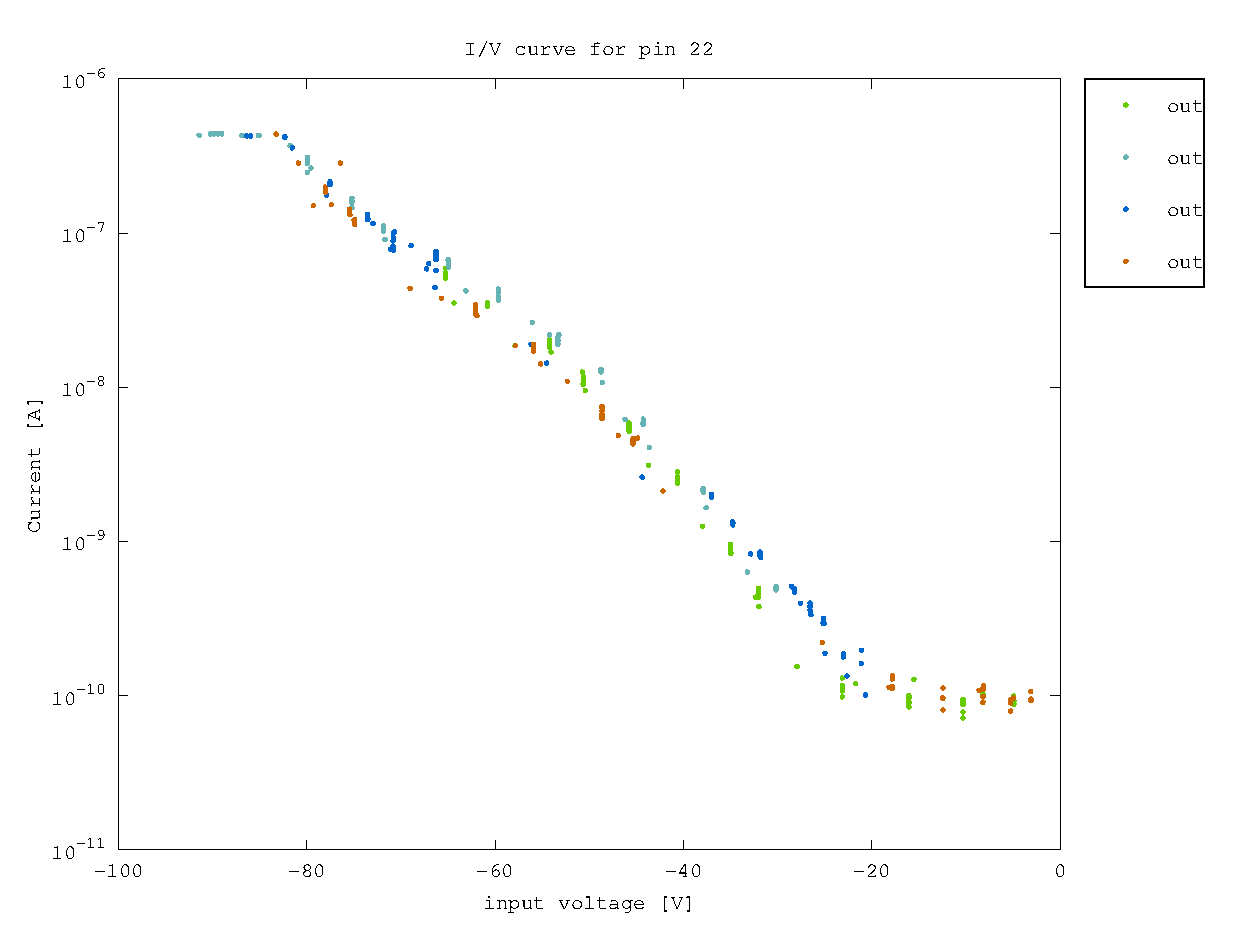
\includegraphics[width=0.7\textwidth]{fig/pin22_slope.eps}
	    \caption[]%
	    {Voltage to current characteristics for a single GaN sensor}    
	    \label{fig:pin22_slope}	
\end{figure}  


\Cref{fig:pin26_slope} shows the behavior of a different sensor. The behavior looks nothing like the previous observations which is most likely due to a defect in the sensor. The green OUT points can not rise to a higher value than approximately $380\,nA$. This limit is caused by the maximum slope on the source follower. In order to extend the reach of the ROIC further, the VBO is used. As concluded in \cref{sssec:VBO_behavior}, the VBO can handle higher voltages because of the higher capacitance. Combining VBO and OUT therefore allows for a large dynamic range. 

\begin{figure}[h]
	    \centering
	    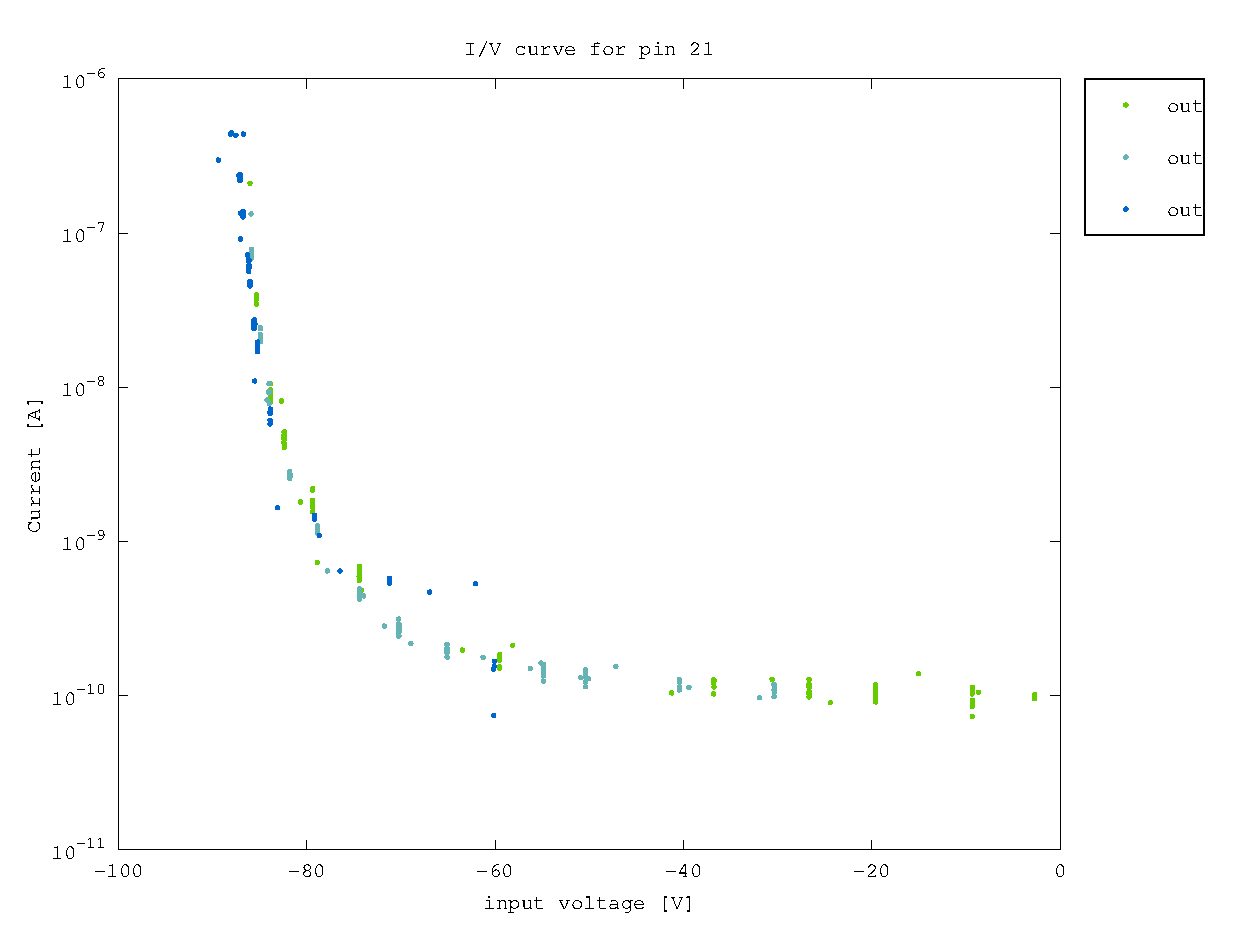
\includegraphics[width=0.7\textwidth]{fig/pin26_slope.eps}
	    \caption[]%
	    {Voltage to current characteristics for a single GaN sensor}    
	    \label{fig:pin26_slope}	
\end{figure}  

\Cref{fig:pin18_slope} and \cref{fig:pin18_slope_lin} show plots for a sensor that is illuminated by a UV source. One can see that the dark current has a steeper slope than the UV light. This means that a clear difference is oberservable for low bias voltages, but the UV loses significance when the dark current increases to higher levels.

\begin{figure}[h]
	    \centering
        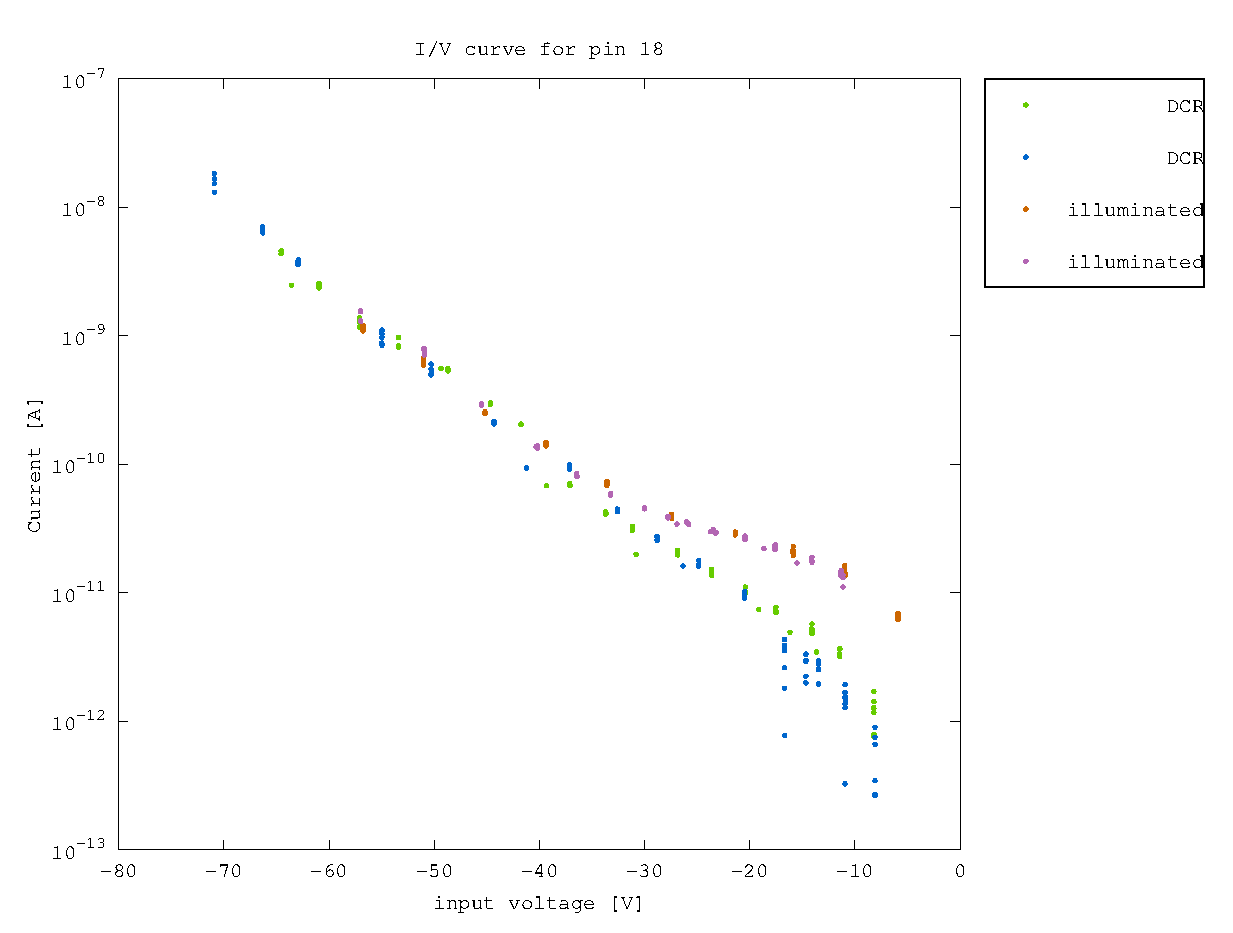
\includegraphics[width=0.7\textwidth]{fig/pin18_slope_UV.eps}
	    \caption[]%
	    {Voltage to current characteristics for a single GaN sensor}    
	    \label{fig:pin18_slope}	
\end{figure}  

\begin{figure}[h]
	    \centering
        \includegraphics[width=0.7\textwidth]{fig/pin18_slope_lin_UV.eps}
	    \caption[]%
	    {Voltage to current characteristics for a single GaN sensor}    
	    \label{fig:pin18_slope_lin}	
\end{figure}  

\clearpage
\subsection{Very high bias voltage}\label{ssec:very_high_bias_voltage}
Besides the $I/V$ measurements, a second observation was made. Specifically, the performance of the ROIC with the GaN sensors for very high bias voltages between 90 and $100\,V$. When the amount of current reaches a certain level, the ROIC is no longer able to maintain it's reset values. This means that during reset, the op amp inside the RIOC is not able to keep up with current produced in the GaN sensor. This causes the input of the integrator to rise to the point that the voltage limiter kicks in. There are two things happening here. This means that the ROIC is no longer functioning. There is a second more problematic effect however. When this modus is kept for to long and/or at a voltage that is too high, the ROIC creates a spark. After that the ROIC is no longer useable. Because of this, three ROICs where damaged. A photo of the inside of the three packaged chips is shown in \cref{fig:burned_chips}. The burns on the chips are on different wires, but for all chips, the burned wire is is the input of the channel that was used at that time. For all three cases, did the wirebond melt and disconnect. However, this is most likely a secondary effect. Especially because the entire chip stops functioning, which should not be the case if only the wirebond fails. Another observation is that the VBO output is pulled to ground, which means that the input is most likely shorted to ground. 


\begin{figure}[H]
	    \centering
	    \includegraphics[width=0.7\textwidth]{fig/burned_chips.JPG}
	    \caption[]%
	    {Inside of packaged ROIC chips after being exposed to too much power}    
	    \label{fig:burned_chips}	
\end{figure}  

This effect is currently the largest constraint to measuring the GaN sensors at high bias voltages, because the ROIC dies before the GaN sensors do.

